%%%%%%%%%%%%%%%%%%%%%%%%%%%%%%%%%%%%%%%%%%%%%%%%%%%%%%%%%%%%%%%%%%%%%%%%%%%%%%%%
% intro.tex: Introduction to the thesis
%%%%%%%%%%%%%%%%%%%%%%%%%%%%%%%%%%%%%%%%%%%%%%%%%%%%%%%%%%%%%%%%%%%%%%%%%%%%%%%%
% Outline:
% - Active matter and active fluids
% - Novel properties: rheology and diffusion
% - Collective phenomena: flocking and giant number fluctuations
%%%%%%%%%%%%%%%%%%%%%%%%%%%%%%%%%%%%%%%%%%%%%%%%%%%%%%%%%%%%%%%%%%%%%%%%%%%%%%%%




\chapter{Introduction}
\label{intro_chapter}
%%%%%%%%%%%%%%%%%%%%%%%%%%%%%%%%%%%%%%%%%%%%%%%%%%%%%%%%%%%%%%%%%%%%%%%%%%%%%%%%

\begin{itemize}

\item Chapter 1 briefly describe the history and significance of active fluid research.

\item Chapter 2 presents the experimental techniques used in this theis.

\item Chapter 3 talks about one of the emergent properties: reduced viscosity. Large portion of  this chapter have been published in \cite{Liu2019}.

\item Chapter 4 talks about another emergent property: giant number fluctuation. This work is under preparation for submission.

\item Chapter 5 presents the study on the transition from disordered state to active turbulence in light-powered bacterial suspensions. This work is conducted with a close collaboration with Yi Peng and Xiang Cheng. Large portions of this chapter has been published in \cite{Peng2020}. Yi Peng, Zhengyang Liu and Xiang Cheng conceived the experiment. Zhengyang Liu constructed the light-powered bacteria. Yi Peng performed the experiment. Zhengyang Liu and Yi Peng did the data analysis. All authors contribute to the model development and writing of the manuscript.

\item Chapter 6 summarizes the contributions of this thesis and provides the outlook on future research.

\item Appendix A shows details of the construction of light-powered \textit{E. coli}.

\item Appendix B provides details of several particle tracking tools I developed.

\item Appendix C shows details of photolithography.

\end{itemize}
%%%%%%%%%%%%%%%%%%%%%%%%%%%%%%%%%%%%%%%%%%%%%%%%%%%%%%%%%%%%%%%%%%%%%%%%%%%%%%%%


%%%%%%%%%%%%%%%%%%%%%%%%%%%%%%%%%%%%%%%%%%%%%%%%%%%%%%%%%%%%%%%%%%%%%%%%%%%%%%%%
\section{Active Matter and Active Fluids}
\label{active-fluids}

Active matter denotes a large group of active units which utilize ambient energy to achieve motions. Examples include flocking birds, schooling fish, herding beasts and even human crowds, down to actin filaments powered by motor proteins, bacteria and chemical reaction driven particles
\cite{Toner2005, Ramaswamy2010, Vicsek2012, Marchetti2013, Saintillan2013, Bechinger2016, Julicher2007}. The concept roots from a broader class of matter: soft matter, which includes polymers, surfactants and colloidal grains and shares common properties such as complexity and flexibility
\cite{DeGennes1992}. Like soft matter, active matter is also complex and flexible. What makes them more complex is the self-propulsion of each individual constituent, which endows them with more intrguing and counter-intuitive properties, challenging our understandings \cite{Glotzer2015}.

\begin{figure}[!htbp]
	\begin{center}
	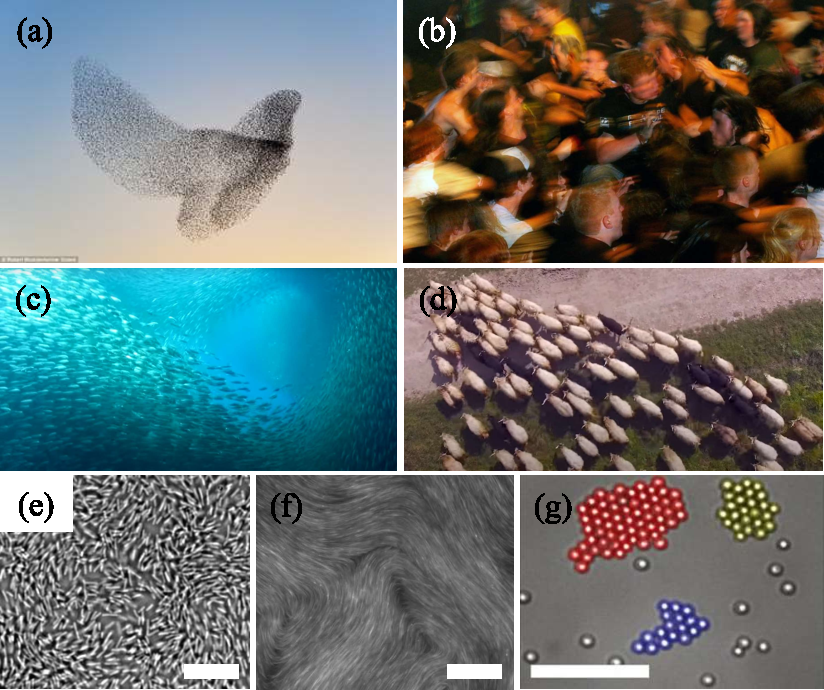
\includegraphics[width=5.5 in]{Figs/1-Intro/1.pdf}
	%select pdftexify command to run jpg or pdf files
	\end{center}
	\caption[Figure 1.1: ]
	{
	\textbf{Examples of living matters and active fluids.}
  (a) Flocking birds, (b) people in a mosh pit at heavy metal converts, (c) schooling fish, (d) herding sheeps, (e) swarming bacteria (f) microtubule and (g) clustering active Janus particles.
  Scalebars in (e) and (g) are 10 \textmu m. Scalebar in (f) is 200 \textmu m. Images courtesy of Robert Wolstenhome (a), Ulrike Biets (b) \cite{Silverberg2013}, biographic (c, d), DeCamp (f) \cite{DeCamp2015} and Palacci (g) \cite{Palacci2013}.
	}
	\label{fig:living-matter-examples}
\end{figure}

Active fluids, sometimes referred to as active gels, are suspensions of active agents such as cells, particles and biological macromolecules that are capable of utilizing chemical energy to sustain their self-propulsion. They are a subset of active matter, and the "fluids" in the name suggests the important role of the viscous hydrodynamic interaction and stress, in contrast to dry active matter \cite{Marchetti2013}. The first glimmering of active fluids dates back to 1969, when Finlayson and Scriven found that motion could spontaneously set in a previously still material without the intervention of outside forces, due to composition-dependent stress \cite{Finlayson1969}. However, the study on active fluids did not bloom, until 26 year later, when the seminal paper on modeling collective flocks came out \cite{Vicsek1995}. From then on, physicists are getting unprecedentedly intereted in biological phenomena, leading to the emergence of a new field of study - active fluids.

Early accomplishments in the research of active fluids include two successful theoretical predictions on the abnormal rheology and the spontaneous active turbulence \cite{Hatwalne2004, Simha2002}, which were then demonstrated in quite a few experiments
\cite{Dombrowski2004, Wensink2012, Rafai2010, Sokolov2009, Gachelin2013, Lopez2015}. From these beginnings, the field has been enjoying a vibrant interplay between experiment and theory, and more complex environment and geometrical constraints have been investigated \cite{Ramaswamy2019}. As of now, the study of active fluids has provided us with a good qualitative understanding of some biological processes, such as how active turbulence enhances nutrient transport.

There are two promising directions in active fluids. One is to get quantitative understanding of the novel properties.  These works will not only provide more accurate predictions on new systems, but also guide the engineering of artificial robots that can perform tasks in complex environment, such as drug delivery. Another direction is to invite chemistry and biology to collaborate on this highly interdisciplinary subject. A complete understanding of the behavior and properties of living systems will require the knowledge of biochemical signaling, which opens the door of an ambitious mission: elucidating tissue dynamics and developmental biology \cite{Marchetti2013, Curatolo2020}. The works that are to be described in Sec.~\ref{rheology-of-bacterial-suspensions-under-confinement},
\ref{giant-number-fluctuations-in-3-dimensional-space} and \ref{the-emergence-of-active-turbulence} are along the first direction: seeking more quantitative understanding of rheology and active turbulence of active fluids.



\section{Novel Properties}
\label{emergent-properties}
Active fluids exhibit novel properties such as reduced viscosity and enhanced diffusion  \cite{Ramaswamy2010}. The reduced viscosity is induced by the force excerted by the swimming mechanisms of the active agents, such as bacteria and algae \cite{Saintillan2018}. And the enhanced diffusion is attributed to the interaction - steric collision or hydrodynamic perturbation - between tracer particles and swimmers
\cite{Wu2000, Peng2016, Caspi2000, Morozov2014, Patteson2016, Leptos2009,
 Yang2016, Valeriani2011, Kurtuldu2011}.
In this section, the existing works regarding rheology and diffusion in active fluids are reviewed, and motivations for investigating the rheology of bacterial suspensions under confinement (Chap.~\ref{rheology-of-bacterial-suspensions-under-confinement}) will be discussed.


\begin{figure}[!htbp]
	\begin{center}
	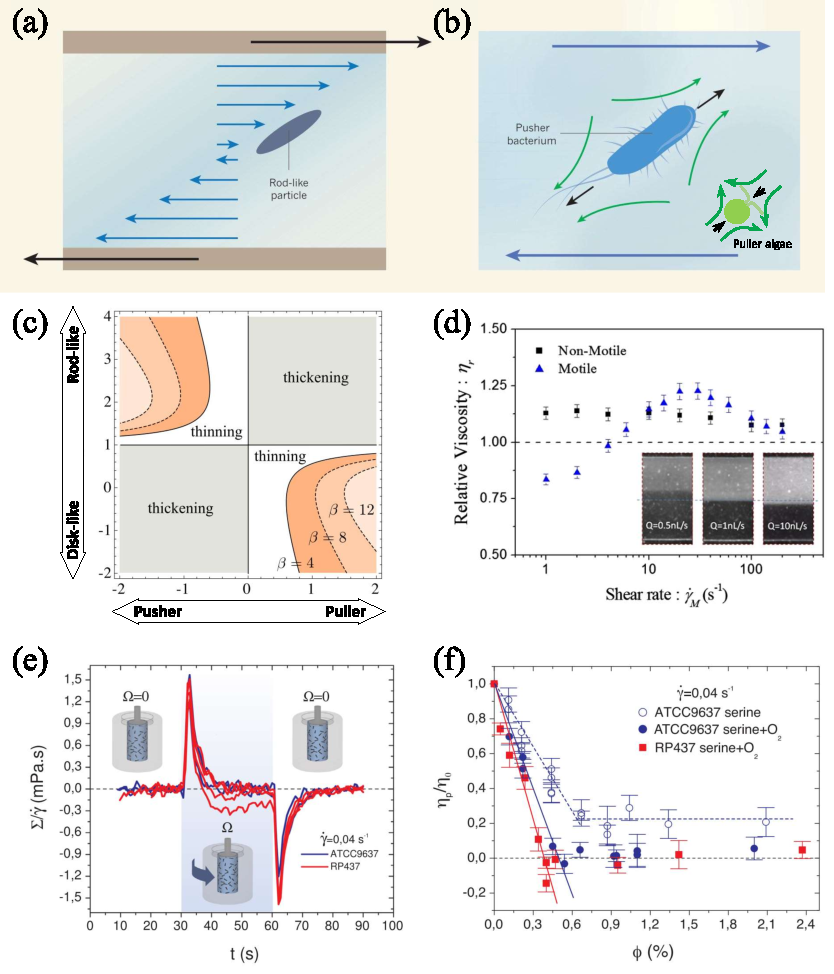
\includegraphics[width=5.5 in]{Figs/1-Intro/2.pdf}
	%select pdftexify command to run jpg or pdf files
	\end{center}
	\caption[Figure 1.2: ]
	{
	\textbf{Rheology of active fluids.}
	(a) The preferred orientation of the bacterium is along the extensile flow.
	(b) The most common pushers and pullers in nature: bacterium and algae, and their corresponding far field flow.
	(c) Rheological effect phase diagram of swimmer shape and swimming mechanism.
	(d) Non-Newtonian behavior of \textit{E. coli} suspensions.
	(e) Stress response of \textit{E. coli} suspensions in a modified Couette concentric cylinder rheometer.
	(f) Viscosity of \textit{E. coli} suspensions at various volume fractions.
	Image courtesy of Marchetti (a, b) \cite{Marchetti2015}, Giomi (c) \cite{Giomi2010}, Gachelin (d) \cite{Gachelin2013} and Lopez (e, f) \cite{Lopez2015}.
	}
	\label{fig:rheology-of-active-fluids}
\end{figure}

\subsection{Rheology}
\label{sec:rheology}
Viscosity of a fluid can be understood as its resistence to flow. When flowing, fluid elements move relative to others, resulting in energy dissipation due to friction. The more energy is required, the more "viscous" the fluid is known to be. A suspension
of passive particles is always more viscous than its suspending fluid, a fact that was first formulated by Einstein in 1906 \cite{Einstein1906}. Recently, the study of active fluids revealed that active particles modify the viscosity of their suspending fluids in a different and interesting way.

In 2004, Hatwalne et al. predicted that micro-swimmers, depending on their self-propelling mechanisms, can modify the suspension viscosity in different ways \cite{Hatwalne2004}. Most common micro-swimmers, such as unicellular microorganisms, can be classified into two types: pushers and pullers, based on the far field flow they generate. Fig.~\ref{fig:rheology-of-active-fluids}b illustrates the most common pushers and pullers in nature: bacterium and algae. If one puts a elongated rod-like bacterium in a simple shear flow, as illustrated in Fig.~\ref{fig:rheology-of-active-fluids}a, the preferred orientation of the bacterium is along the extensile flow \cite{Forster1974}. Such an orientation makes the flow generate by the swimming bacterium coincide with the imposed shear flow, and thus compensating the viscous dissipation of energy, which effectively reduces the viscosity. In contrast, in the case of puller swimmers, such an orientation makes opposites the directions of swimming induced flow and imposed shear flow, which enhances the visocity.

Their prediction was confirmed by numerical solutions of the theory \cite{Cates2008, Giomi2010} and experiments \cite{Sokolov2009, Gachelin2013, Lopez2015}. Cates et al. reached at the same conclusions as Hatwalne et al. did: while contractile gels exhibit a divergence of apparent viscosity, extensile gels show a zero-viscosity phase. Giomi et al., on top of these results, emphasized the important role of particle shape. They showed, in their numerical study, an rheological equivalence between rod-like pusher swimmers and disk-like puller swimmers (see Fig.~\ref{fig:rheology-of-active-fluids}c). In particular, they predicted a thickening effect of spherical puller swimmers (corresponds to the 0 shape parameter in Fig.~\ref{fig:rheology-of-active-fluids}c). This prediction was later on challenged by another theory in the framework of swim stress, which predicts a viscosity reduction of a spherical pusher swimmer suspension
\cite{Takatori2017}. Due to the difficulty of synthesizing large amount of artificial swimmers, this debate has not been resolved yet. However, with the rapid development of synthesizing techniques \cite{Palacci2013, Bricard2013}, it is getting more promising that we will resolve it, and formulate a more complete understanding on how active swimmers modify the rheology.

Experimental confirmation of these predictions posed challenges on traditional rheometries due to the tiny shear stress that is required to be measured. As a result, new rheometries are needed \cite{Marchetti2015}. In 2009, Sokolov and Aranson came up with an innovative way of measuring the such tiny stress \cite{Sokolov2009}. By moving a probe in a suspension of \textit{Bacillus subtilis} bacteria, a pusher type swimmer, they generated a large vortex. By studying the decay of the vortex, they got a measure of the viscosity. For the first time, they experimentally confirmed that pusher swimmers reduced the viscosity (see their results in Fig.~\ref{fig:rheology-of-active-fluids}d). In 2013, Gachelin et al. adopted a microfluidic viscometer to measure the viscosity of suspensions of \textit{Escherichia coli} bacteria, another pusher type swimmer \cite{Gachelin2013}. They confirmed again the viscosity reduction. A more remarkable finding is the non-newtonian behavior: the viscosity was reduced at low shear rate, but was enhanced at high shear rate. This observation suggested that it is the competation between bacterium intrinsic shear rate and the impose flow shear rate that determines how the viscosity is modified. In 2015, Lopez et al. published arguably the most important experimental work on the rheology of active fluids, which showed that the apparent viscosity of an \textit{E. coli} suspension can be reduced to zero if the swimming activity is sufficiently high \cite{Lopez2015}. The authors modified an old-fashioned Couette concentric cylinders, where the outer cylinder was set to rotate at a fixed rate and the torque on the inner cylinder was measured. The high sensitivity was achieved by using a string that was highly sensitive to torque to hang the inner cylinder, so that a stress, as small as that generated by bacterial suspensions, can be detected (see their rheometer and results in Fig.~\ref{fig:rheology-of-active-fluids}e-f). The authors termed their zero-viscosity suspensions ``superfluids''.

Despite the great progress on the rheology of active fluids made so far, there remains complexity that is not readily understood. Confinement, or more generally boundary conditions or geometry, is one of the leading factors that contributes to this complexity. The behavior of active particles can be altered greatly by confinement. In 2005, Voituriez et al. showed theoretically that a spontaneous flow transition from a homogeneous immobile state could happen in active polar gel under confinement \cite{Voituriez2005}. Such spontaneous flow transition was confirmed in both numerical and experimental studies \cite{Ravnik2013, Wioland2016, Wu2017}. The complexity introduced by geometry was also manifested by the experiments where single bacterial vortex was stabilized by confinement \cite{Woodhouse2012, Wioland2013, Lushi2014} and where asymmetric gears were powered by swimming bacteria
\cite{Sokolov2010, Hamby2018}. The effect of confinement on the rheology of active fluids was first studied theoretically based a kinetic theory \cite{Alonso-Matilla2016} and a generalized Navier-Stokes model \cite{Somka2017}. In this thesis, I will present the first experimental study on active fluid rheology using bacterial suspensions
(Chap.~\ref{rheology-of-bacterial-suspensions-under-confinement}). The fact that our experimental results agreed with neither theory manifested the complexity and the lack of understanding of active fluids. Together with the experimental results, we provided a heuristic model that qualitatively captured the rheological properties and hope to stimulate further theoretical studies on this matter.




\begin{figure}[!htbp]
	\begin{center}
	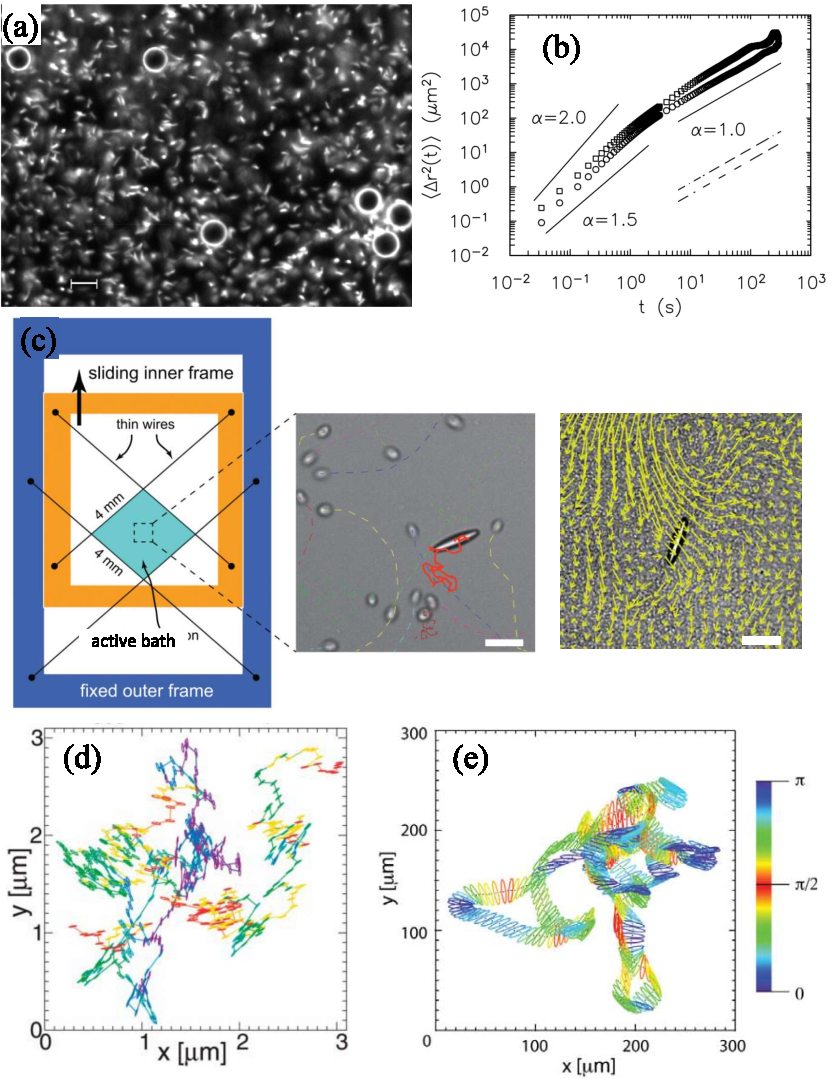
\includegraphics[height=5.5 in]{Figs/1-Intro/3.pdf}
	%select pdftexify command to run jpg or pdf files
	\end{center}
	\caption[Figure 1.3:]
	{
	\textbf{Diffusion of passive tracers in an active bath.}
	(a) 10 \textmu m diameter PS particles suspended in a bath of \text{E. coli}
	(b) Mean squared displacement (MSD) of tracer paticles as a function of lag time.
	(c) Free-standing film setup adopted by Peng et al. and Yang et al. (left)\cite{Peng2016, Yang2016}. A microscopic image of ellipsoidal PS particle suspending in \textit{C. reinhardtii} (middle) and \textit{E. coli} (right) baths. Scale bar: 20 \textmu m.
	(d) and (e) present both the translational and orientational trajectories of ellipsoids diffusion in water and \textit{E. coli} bath, respectively.
	Image courtesy Wu (a, b) \cite{Wu2000}, Yang (c) \cite{Yang2016}, Han (d) \cite{Han2006} and Peng (e) \cite{Peng2016}.
	}
	\label{fig:diffusion-in-active-fluids}
\end{figure}

\subsection{Diffusion}
\label{sec:diffusion}
The diffusion of passive particles in active fluids, such as nutrients and signaling molecules, are significantly enhanced. Such enhancement has been shown to have great biological and ecological importance \cite{Wu2000, Kurtuldu2011, Morozov2014}, as well as to provide a useful tool of probing novel properties of active fluids \cite{Squires2010}. Unlike the study of rheology, which was initiated by theoretical prediction, the study of enhanced diffusion started from an experiment.

In 2000, Wu and Libchaber studied the diffusion of spherical polystyrene particles in a bath of actively swimming \textit{E. coli} \cite{Wu2000} (see Fig.~\ref{fig:diffusion-in-active-fluids}a for their experimental system). They characterized the diffusion of the tracer particles by measuring their means squared displacement (MSD) (see Fig.~\ref{fig:diffusion-in-active-fluids}b for typical MSD data), and reported two findings: 1) the MSD exhibits a superdiffusive regime at short time, which is followed by a diffusive regime at longer time; 2) the effective temperature, backed up from effective diffusion coefficient using Stokes-Einstein equation, is several order of magnitude larger than room temperature. Their qualitative findings were confirmed by computational \cite{Underhill2008, Lin2011}, theoretical \cite{Golestanian2009} and other experimental studies
\cite{Chen2007, Leptos2009, Mino2011, Kurtuldu2011, Patteson2016}. A remarkable progress towards quantitative understanding was made by Mino et al., who experimentally identified that the enhancement of diffusivity is proportional to the "activity flux" (defined as concentration multiplied by the mean velocity of swimmers). This model was further developed to capture the experimental result more accurately and to account for more complex conditions \cite{Mino2013, Kasyap2014, Morozov2014}.

Although a lot of progress has been made on understanding diffusion isotropic particles (spheres) in an active bath, how anisotropic particles diffuse remained largely unexplored. Yet, the diffusion of anisotropic particles has both fundamental and application significance. On the one hand, it was shown that the Brownian motion (i.e. in a passive bath) of anisotropic particles exhibited a subtle interplay between orientational and translational motions \cite{Han2006}. Previous studies preferred to consider an active bath equivalent to a high temperature passive bath \cite{Wu2000}, and it was shown to be a good equivalence for isotropic particles. A fundamentally interesting question to ask is: does active bath also alters the interplay between orientational and translational motions? The answer is yes, and we will see that this interplay is specific to swimming mechanisms. On the other hand, few particles or molecules in nature are perfectly isotropic. Generalizing the enhanced diffusion to anisotropic particles will have significant impact on applying this knowledge to real world problems. In 2016, Peng et al. studied the diffusion of polystyrene ellipsoids in a quasi-2D free-standing soap film of \textit{E. coli} bath (see setup schematic in Fig.~\ref{fig:diffusion-in-active-fluids}c) \cite{Peng2016}. In contrast to the pure Brownian motion, where ellipsoids preferred to diffuse along their major axes \cite{Han2006}, they found that an active bath forced
the ellipsoids to move primarily along the minor axes (see Fig.~\ref{fig:diffusion-in-active-fluids}d-e for a comparison). This phenomenon was explained by considering the far-field dipole flow of a single \textit{E. coli} bacterium. An interesting prediction naturally arises: in a bath of puller swimmers, whose far-field flow is opposite to that of pushers, the diffusion of ellisoidal tracers should be primarily along the major axes. This prediction was later on proved experimentally by Yang et al. \cite{Yang2016} in a green algae \textit{C. reinhardtii} bath and I was involved in this work. Due to the fact that my contribution was relatively small to this work, I will not provide more details about it in my thesis. However, readers interested are encouraged to find out more in our original paper \cite{Yang2016}.





\section{Collective Motion and Giant Number Fluctuations}
Collective motion is defined as an emergent directed movement in a large number of animals or particles, which are capable of moving on their own. In the seminal paper by Reynolds published in 1987, he tried to use a simulation approach, rather than scripting the paths beforehand, to generate vivid motions of animals in computer graphics \cite{Reynolds1987}. This idea has soon evoked enormous research interest of physicists because a seemingly universal animal behavior was found in animals across different length scales: up to large animals as birds and fish, and down to small insects and micro organisms.

In this section, we first review recent progresses on understanding the collective motions in various living and non-living systems. Our research on ``imaging the emergence of active turbulence'' will be motivated
(detailed in Chap.~\ref{the-emergence-of-active-turbulence}). Then, I will describe an important consequence of the collective phenomena: giant number fluctuations (GNF), which is regarded as a landmark phenomenon of collectively moving particles. I will motivate our research on ``giant number fluctuations in 3-dimensional bacterial suspensions'' in this section, and the details of this research will be shown in Chap.~\ref{giant-number-fluctuations-in-3-dimensional-space}.

\begin{figure}[!htbp]
	\begin{center}
	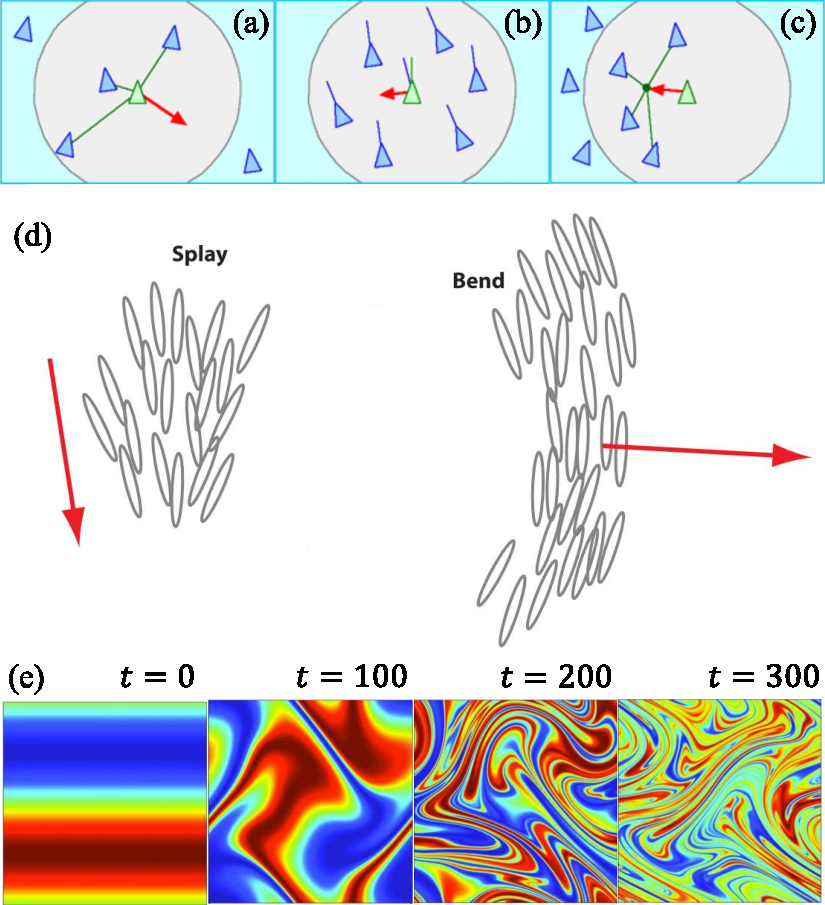
\includegraphics[width=5.5 in]{Figs/1-Intro/4.pdf}
	%select pdftexify command to run jpg or pdf files
	\end{center}
	\caption[Figure 1.4:]
	{
	\textbf{Illustrations of existing models and theories of collective motions.}
	(a)-(c) Reynolds’ “boids” model obeying the rules of separation (a), alignment (b) and cohesion (c).
	(d) Nematic self-propelled particle model, displaying splay (left) and bend (right) instability.
	(e) Simulation of efficient fluid mixing driven by active pusher swimmers.
	Image courtesy of Reynolds (a-c) \cite{Reynolds1987}, Ramaswamy (d) \cite{Ramaswamy2010} and Saintillan (e) \cite{Saintillan2008b}.
	}
	\label{fig:models-of-collective-motions}
\end{figure}

\subsection{Collective Motion}
The research on collective motion dates back to the 1980s, when flocking birds, schooling fish, herding beasts and even human crowds (Fig.~\ref{fig:living-matter-examples}a-d) were regarded as an orientationally ordered phase of living matter, in analogy with ferromagnetic spins
\cite{Reynolds1987, Vicsek1995, Narayan2007, Ward2008, Ballerini2008, Silverberg2013}. Besides macroscopic systems mentioned above, smaller and more laboratory accessible model systems have joined this family and have been studied extensively. As examples, actin filaments and bacteria exhibit turbulence-like swirling patterns, and synthetic active colloids form dynamic clusters (Fig.~\ref{fig:living-matter-examples}e-g)
\cite{Dunkel2013, Wensink2012, Buttinoni2013, Palacci2013, Sanchez2012, Schaller2010, Sokolov2007}.


While being fascinated by the patterns formed by collectively moving animals or particles, researchers are trying to come up with rules, models and theories to explain and predict this process. There is a vast literature trying to understand collective motions in different systems from various approaches. To get an idea of how extensively it has been studied, Ref~\cite{Reynolds1987} by Reynolds has been cited more than 10,000 times so far. I will briefly review the attempts to model collective motion, which are most relevant to our research that will be detailed in the following chapters. A more comprehensive review on the studies of collective motions can be found in the review paper by Vicsek \cite{Vicsek2012}. In 1987, Reynolds came up with arguably the first set of rules to capture the features of collective motions, based on a simple self-propelled particle model. Three rules were set into the system: seperation, alignment and cohesion, as illustrated in Fig.~\ref{fig:models-of-collective-motions}a-c, where  the blue and green triangles in are the actively moving particles in his simulation, called ``boids'' \cite{Reynolds1987}. In 1995, Vicsek modified Reynolds' model by replacing the separation and cohesion rule with a random perturbation in the velocity of each particle, while keeping the alignment rule, which dictates one particle to always point to the same direction as its neighbors \cite{Vicsek1995}. Due to the simpler and more robust rules compared to Reynolds' model, Vicsek's model was able to simulate huge flocks. In later studies, the Vicsek Model has become a standard model where properties of collective motions are explored
\cite{Gregoire2004, Chate2008, Ginelli2010, Ngo2014, Mahault2019}. Despite the success of discrete and finite system simulation in understanding 2D collective motions, it was challenging to study long range, long time and higher dimensional dynamics using such approach. In 1995, Toner and Tu wrote down a continuum equation of motion for a ``large universality class of models'' such as the Vicsek Model based on symmetry and conservation arguments \cite{Toner1995}. In 2002, Simha and Ramaswamy made the first attempt to address hydrodynamic effect in self-propelled particle suspensions \cite{Simha2002}. Within the framework of liquid crystal physics, they formulated an equation of motion with hydrodynamic terms to account for the
``flow-alignment'' effect \cite{Forster1974}. The inclusion of hydrodynamic effects turned out to be very important, because it directly accounted for phenomena in bacterial suspensions, the largest group of prokaryotic organisms and the most studied model active system. Their theory captures several aspects of bacterial suspensions well, including the emergence of active turbulence and giant number fluctuations as a consequence of the bend instability of an ordered state (illustrated in Fig.~\ref{fig:models-of-collective-motions}d). In 2008, Saintillan and Shelly adapted kinetic theories, which were previously used to study polymers, to study the suspensions of self-propelled particles \cite{Saintillan2008a, Saintillan2008b}. Their theory generalized the predictions by Simha and Ramaswamy by predicting that, in addition to ordered state, a disordered state is also unstable and can evolve into a turbulent state. Moreover, they made interesting investigations on the nonlinear effects, such as pattern formation and efficient fluid mixing. Fig.~\ref{fig:models-of-collective-motions}e shows one instance of their simulation on the evolution of fluid mixing driven by active pusher swimmers. There are other attempts to model the collective motion and its consequences that I haven't included. For a more comprehensive review of both theoretical and experimental advances, see the review papers
\cite{Ramaswamy2010, Koch2011, Marchetti2013}.

As of today, these universal patterns can be qualitatively reproduced by simple models with collision rules and noise. And quantitative description is developing with more observations available, which is bound to have impactful applications, including understanding the reaction of panic crowd and predicting the migration of fish schools
\cite{Vicsek2012}.

In my research, bacterial suspensions are the model system. In such system, the collective motion is usually manifested by the emergence of ``active turbulence'', where vigorously swimming bacteria are stirring the fluid and generating vortex- and jet-like patterns, reminiscent of high Reynolds number turbulence \cite{Dombrowski2004, Sokolov2007, Sokolov2009,
Sokolov2012, Ishikawa2011, Wensink2012, Dunkel2013, Peng2020}.
The onset of large scale collective motions in bacterial suspensions has been regarded as a disorder-order phase transition, where critical conditions at which the transition should happen have been predicted by various theoretical works \cite{Baskaran2009, Koch2011, Marchetti2013, Saintillan2015}.
In constrast to the abundance of theoretical predictions, definitive experiments that can quantitatively verify them are  still lacking \cite{Koch2011, Saintillan2015}.
To fill this gap, I worked closely with my colleague Dr. Yi Peng on systematically measuring the critical conditions of this transition. The result will be presented in Chap.~\ref{the-emergence-of-active-turbulence}.

 \begin{figure}[h]
 	\begin{center}
 	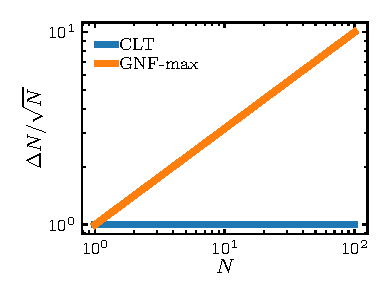
\includegraphics[width=5 in]{Figs/1-Intro/GNF/GNF-illustration.pdf}
 	\end{center}
 	\caption[Illustrations of giant number fluctuations]
 	{
	\textbf{Illustrations of giant number fluctuations.}
	(a)-(b) a 2-particle system and a 3-particle system, along with the probabilities and the standard deviations of each configuration.
	(c) The most extreme configuration of 2-particle and 3-particle systems.
	(d) Number fluctuation curves, where standard deviation of number of particles rescaled by the square root of mean number $\Delta N/\sqrt N$ is plotted against the mean number $N$. The scaling exponent of these curves, denoted as $\alpha$, measures the magnitude of GNF.
 	}
 	\label{fig:GNF-illustration}
 \end{figure}

\subsection{Giant Number Fluctuations}
Active particles displays transient large scale inhomogeneity even in a \textit{statistically homogeneous and stationary state}.
Such a phenomenon is referred to as \textit{giant number fluctuations} (GNF). Formally, it is defined as the anomalously strong dependence of the variance of the number of particles on the mean number.
GNF was predicted by a number of early theoretical works \cite{Toner1995, Toner1998,
Tu1998, Simha2002, Ramaswamy2003, Saintillan2008a, Saintillan2008b, Ramaswamy2010}, and was confirmed by observations in computational models
\cite{Mishra2006, Chate2008, Dey2012, Saintillan2012, Ngo2014, Mahault2019} and experimental realizations
\cite{Narayan2007, Aranson2008, Zhang2010, Deseigne2010, Schaller2013, Palacci2013,
Kawaguchi2017, Nishiguchi2017, Karani2019}. Over the past two decades, GNF has been shown to be universal across multiple length scales and is now being regarded as a landmark of collectively moving active particle systems. Despite the many studies on this universal phenomenon, a quantitative understanding is still lacking. Specifically, the scaling exponent of the variance of the number of particles on the mean number has not been measured in a definite way. In this section, I will review the attempts that have been made to fill these gaps and motivate our reseach on GNF, which will be described in detail in Chap.~\ref{giant-number-fluctuations-in-3-dimensional-space}.

A particle system in thermal equilibrium obeys central limit theorem, which states that when the size of a system gets very large, the fluctuation of particle number is negligible. More quantitatively, the number fluctuations represented by the standard deviation $\Delta N$ scales with the square root mean number $N^{0.5}$. From a statistical mechanics point of view, the configuration of a particle system in equilibrium can be determined by randomly assigning states to each particle and find the most probable configuration. Fig.~\ref{fig:GNF-illustration}a-b shows all the possible configures of a 2-particle system and a 3-particle system, with corresponding probability of each configuration shown on the side. Each particle has only two possible states: ``left'' and ``right''. If we keep increasing the particle number $N$ and calculte the emsemble average of the standard deviation $\Delta N$, the resulting number fluctuation curve ($\Delta N/\sqrt N$ vs. $N$) will be a flat line, as shown by the blue line in Fig.~\ref{fig:GNF-illustration}d. This curve describes the number fluctuations in equilibrium systems.

\begin{figure}[htbp]
 \begin{center}
 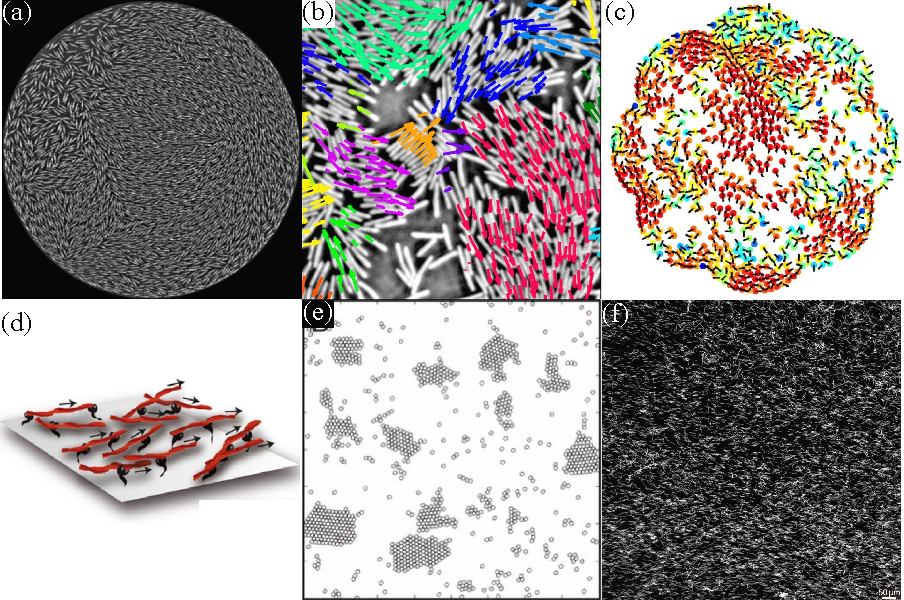
\includegraphics[height=6 in]{Figs/1-Intro/GNF/GNF-experiments.pdf}
 \end{center}
 \caption[Experimental realizations of active systems showing giant number fluctuations]
 {
 \textbf{Experimental realizations of active systems showing giant number fluctuations.}
 (a) Granular rods driven by a vibrating surface underneath them.
 (b) Swarming \textit{B. subtilis} bacteria on semi-solid media.
 (c) Vibrated disks.
 (d) Actin filaments powered by motor proteins.
 (e) Janus particles powered by chemical reactions.
 (f) Swimming \textit{E. coli} confined in quasi-2D glass chambers.
 Image courtesy of Narayan \cite{Narayan2007}, Zhang \cite{Zhang2010}, Deseigne \cite{Deseigne2010}, Schaller \cite{Schaller2013}, Palacci \cite{Palacci2013} and Nishiguchi \cite{Nishiguchi2017}.
 }
 \label{fig:GNF-experiments}
\end{figure}

In contrast, an active particle suspension is constantly driven out of equilibrium by the energy flux transduced by the micro-swimmers.
As a result, acitve systems deviate from the central limit theorem, with $\Delta N$ scales faster than $\sqrt N$.
Consider the most extreme case in the ``left-right'' system, where the probability of all particles have the same state is 1, as shown in Fig.~\ref{fig:GNF-illustration}c.
If we plot the number fluctuation curve ($\Delta N/\sqrt N$ vs. $N$) for such a system, the curve will show a scaling exponent 0.5, as shown by the orange line in Fig.~\ref{fig:GNF-illustration}d.
We define the excess scaling exponent as the measure of the magnitude of GNF, and use $\alpha$ to denote it.
In a typical active system exhibiting GNF, we have $\Delta N \sim N^{0.5+\alpha}$ where $0.5\ge\alpha>0$, as indicated by the gray region (GNF) in Fig.~\ref{fig:GNF-illustration}d.

Many experimental attempts has been made to measure $\alpha$. In 2007, Narayan et al. did the first experiment focusing on GNF with shaking granular rods, which the authors termed a "fluidized monolayer of rods" (Fig.~\ref{fig:GNF-experiments}a)\cite{Narayan2007}. The $\alpha$ measured by them was as large as 0.5, the largest possible value of $\alpha$. And they also observed a much slower decay of the temporal autocorrelation of the density fluctuations, which directly confirmed the theoretical predictions made by Ramaswamy et al. \cite{Ramaswamy2003}.
Similar experiments, where macroscopic granules were driven by a vibrating surface, have also been conducted by Kudrolli et al. \cite{Kudrolli2008} and Deseigne et al. (Fig.~\ref{fig:GNF-experiments}c)\cite{Deseigne2010}. These authors reported $\alpha$ to be 0.16 and 0.22, respectively.
Quantitative assessment of GNF in biological systems was first done in 2010 by Zhang et al. on swarming \textit{B. subtilis} bacteria on semi-solid agar media (Fig.~\ref{fig:GNF-experiments}b) \cite{Zhang2010}.
The claimed to have identified GNF in a biological system and reported the $\alpha$ to be around 0.25.
Their work was followed by more microscopic measurements, in both biological and synthetic active systems \cite{Schaller2013, Palacci2013, Kawaguchi2017, Nishiguchi2017, Karani2019}.
Some of the systems studied in these works are also shown in Fig.~\ref{fig:GNF-experiments}, including actin filaments powered by motor proteins (d), Janus particles powered by chemical reactions (e) and swimming \textit{E. coli} bacteria (f).
The alpha reported by these works range from 0.13 to 0.3.
Table.~\ref{table:alpha-values} shows all the $\alpha$ values reported by previous experiments described above.

\begin{table}[h]
	\centering
	\spacerows{1.2}
	\begin{tabular}{  lccc m{2in} }
		\toprule
		Author              & Year & Dimensionality & $\alpha$ & System \\\midrule
		Narayan et al.      & 2007 & 2-D            &  0.5     & granular rods on vibrating surface \\
		Kudrolli et al.     & 2008 & 2-D            &  0.16    & granular rods on vibrating surface \\
		Deseigne et al.     & 2010 & 2-D            &  0.22    & granular disks on vibrating surface \\
		Zhang et al.        & 2010 & 2-D            &  0.25    & swarming \textit{B. subtilis} bacteria on semi-solid agar media \\
		Schaller et al.     & 2013 & 2-D            &  0.3     & actin filaments powered by motor proteins \\
		Palacci et al.      & 2013 & 2-D            &  0.38    & Janus particles powered by chemical reactions \\
		Kawaguchi et al.    & 2017 & 2-D            &  0.25    & neural progenitor cells \\
		Nishiguchi et al.   & 2017 & 2-D            &  0.13    & swimming \textit{E. coli} bacteria \\
		Karani et al.       & 2019 & 2-D            &  0.35    & Quincke particles powered by electric fields \\
		\bottomrule
	\end{tabular}
	\caption{$\alpha$ values reported by previous experiments.}
	\label{table:alpha-values}
\end{table}

By summarizing these experimental results, we realize that the $\alpha$ values measured from different systems show significant discrepancies. While $\alpha$ can only take values from 0 to 0.5, the reported values have already ranged from 0.13 to 0.5, which spans almost the whole range of possible values.
Although it is very encouraging to have observed a predicted phenomenon in many different systems across multiple length scales, further advancement of the understandings of this seemingly universal phenomenon relies strongly on more definite measurements. All the previous experiments were conducted in 2-dimensional systems, which were unavoidably affected by frictional walls. Therefore, we conceived a measurement of GNF in a 3-dimensional system, which is free from frictional walls and can provide a more definite value of $\alpha$.

Collectively moving particles form remarkable macroscopic patterns in dense suspensions in forms of complex vortices and jets. Such patterns resemble the classic high Reynolds number turbulence, and has been referred to as meso-scale turbulence or active turbulence \cite{Wensink2012}. Due to this analogy, the quantity that has been widely used in traditional turbulence study --- energy spectra --- has been borrowed to investigate the flow structures of active turbulence
\cite{Ishikawa2011, Saintillan2012, Bratanov2015, Giomi2015, Bardfalvy2019, Linkmann2019, Chatterjee2019, Skultety2020, Peng2020}.
Saintillan et al. computationally studied the energy spectra of 2-dimensional suspensions of rod-like active particles at various volume fractions, and found that at large wavenumber $k$, all volume fraction samples showed a universal scaling exponent $-4$. Such universal behavior broke down at large length scale, when $k$ is small \cite{Saintillan2012}.
% Wensink et al. experimentally measured the energy spectra of \textit{B. subtilis} suspensions and found a good agreement with both self-propelled rod model and continuum theory results \cite{Wensink2012}.
% Bratanov et al. investigated numerically and analytically a continuum description of active turbulence involving a cubic nonlinearity. They found that such a nonlinear term leads to a nonuniversal energy spectra at large scale, defining a new class of turbulent flows \cite{Bratanov2015}.
% I don't really understand this
Using a mean-field theory, Giomi obtained the energy spectra of 2-dimensional active nematics, and found that they decay with the wavenumber $k$ as $k^{-4}$, inconsistency with the numerical result obtained by Saintillan et al. \cite{Giomi2015}.
These results are suggesting an important distinction between the classic turbulence and active turbulence.
As suggested by Bratanov et al., who investigated numerically and analytically a continuum description of active turbulence involving a cubic nonlinearity, active fluids is defining a new class of turbulent flows due to the self-organization of active particles \cite{Bratanov2015}.
Although this distinction has been predicted by a number of theories and simulations, a systematic measurement of energy spectra in active turbulence is lacking.
Moreover importantly, we notice that both energy spectra and GNF describe the scale-dependent properties of an active system. Such analogy indicates connections between the two quantities.
In Chap.~\ref{giant-number-fluctuations-in-3-dimensional-space}, I present a systematic study on both GNF and energy spectra in active suspensions of various volume fractions. I will show that a close connection between GNF and energy spectra indeed exists, which hints the microscopic origin of GNF.

% \subsubsection{Driving force}
%
% The driving force of GNF, especially in wet systems, remains unclear. Elucidating the behavior of collectively moving bacteria has proved to be challenging, because it involves many active constituents interacting with each other and it is impossible to analytically solve for the motions of every single particle. As a result, the advancement of understanding collective motions relies on mesoscopic coarse-graining approaches
% \cite{Simha2002, Ramaswamy2003, Aranson2005, Bertin2006, Aranson2007,
% Baskaran2008, Saintillan2008a, Saintillan2008b, Baskaran2009}
% and agent-based simulations
% \cite{Vicsek1974, Gregoire2004, Mishra2006, Hernandez-Ortiz2005, Chate2008,
% Ginelli2010, Saintillan2012, Dey2012, Ngo2014, Mahault2019}. By comparing the theoretical and computational predictions with experimental observations, we have a chance to find out some correct or close enough assumptions.
%
% Successful comparisons have been made
% Long time tail of concentration autocorrelation (Toner 1998 and Ramaswamy 2003): Narayan 2007 and Schaller 2013
% alpha = 1/d (Ramaswamy 2003): Narayan 2007




%%%%%%%%%%%%%%%%%%%%%%%
